%:-+-+-+- Engendré par : http://math.et.info.free.fr/TikZ/Arbre/
\begin{center}
% Racine en Haut, développement vers le bas
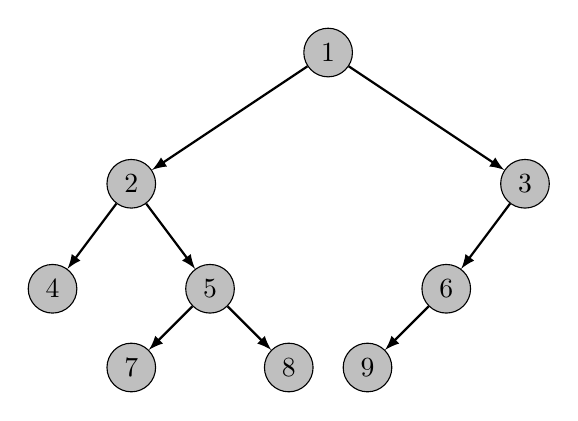
\begin{tikzpicture}[xscale=1,yscale=1]
% Styles (MODIFIABLES)
\tikzstyle{fleche}=[->,>=latex,thick]
\tikzstyle{noeud}=[fill=lightgray,circle,draw]
\tikzstyle{feuille}=[fill=lightgray,circle,draw]
% Dimensions (MODIFIABLES)
\def\DistanceInterNiveaux{1}
\def\DistanceInterFeuilles{2}
% Dimensions calculées (NON MODIFIABLES)
\def\NiveauA{(-0)*\DistanceInterNiveaux}
\def\NiveauB{(-1.6666666666666665)*\DistanceInterNiveaux}
\def\NiveauC{(-3)*\DistanceInterNiveaux}
\def\NiveauD{(-4)*\DistanceInterNiveaux}
\def\InterFeuilles{(1)*\DistanceInterFeuilles}
% Noeuds (MODIFIABLES : Styles et Coefficients d'InterFeuilles)
\node[noeud] (R) at ({(1.75)*\InterFeuilles},{\NiveauA}) {$1$};
\node[noeud] (Ra) at ({(0.5)*\InterFeuilles},{\NiveauB}) {$2$};
\node[feuille] (Raa) at ({(0)*\InterFeuilles},{\NiveauC}) {$4$};
\node[noeud] (Rab) at ({(1)*\InterFeuilles},{\NiveauC}) {$5$};
\node[feuille] (Raba) at ({(0.5)*\InterFeuilles},{\NiveauD}) {$7$};
\node[feuille] (Rabb) at ({(1.5)*\InterFeuilles},{\NiveauD}) {$8$};
\node[noeud] (Rb) at ({(3)*\InterFeuilles},{\NiveauB}) {$3$};
\node[noeud] (Rba) at ({(2.5)*\InterFeuilles},{\NiveauC}) {$6$};
\node[feuille] (Rbaa) at ({(2)*\InterFeuilles},{\NiveauD}) {$9$};
% Arcs (MODIFIABLES : Styles)
\draw[fleche] (R)--(Ra);
\draw[fleche] (Ra)--(Raa);
\draw[fleche] (Ra)--(Rab);
\draw[fleche] (Rab)--(Raba);
\draw[fleche] (Rab)--(Rabb);
\draw[fleche] (R)--(Rb);
\draw[fleche] (Rb)--(Rba);
\draw[fleche] (Rba)--(Rbaa);
\end{tikzpicture}
\end{center}
%:-+-+-+-+- Fin
